\documentclass[conference]{IEEEtran}

\usepackage[dvips]{graphicx}
\usepackage{amsmath,amssymb}
\usepackage{algorithm}
\usepackage{algorithmic}

\begin{document}
\title{Paper Title (Each Word of the Title Should Begin with a Capital Letter with the Exception of Articles and Conjunctions)}
\date{}%date stay empty

\author{
\IEEEauthorblockN{Line 1 - FullName1, FullName2}
\IEEEauthorblockA{Line 2 - Name of organization1 \\ Line 3 - City1, Country1 \\ Line 4 - {Author1, Author2}@domain.edu\\}
\and
\IEEEauthorblockN{FullName3}
\IEEEauthorblockA{Name of organization2 \\ City2, Country2 \\ Author3@domain.edu\\}}
\maketitle

\begin{abstract}
The abstract describes a summary of the paper. In some cases, the authors confuse the abstract with the introduction. In the abstract using of acronyms and abbreviations is undesirable.  
\end{abstract}

\section{Introduction (Heading 1)}
For publication in the section Full Paper, beginning with the Proceedings of FRUCT14, article must be at least 6 pages and no more than 12 pages. Abstracts for performances may be from 1 to 3 pages. Exceeding these volumes is only possible by prior agreement with the organizers of the conference.

In \TeX for program listing is using command $\setminus$\ttfamily ttfamily.

\rmfamily
If you would like to make a cite, place it at the end of sentence before point or comma.

\subsection{Information about authors}
Please place last name after first name, declare them completely. If all the authors work in one place, their names are written with a comma (after last's no comma) in a single column. So a number of columns are equal to number of authors working in different places. Following declare author's place of work (at new line, no comma in the end). Place of work it's only general name of company or university, without name of particular department. On the new line place city and country by comma, and on the last line -- email (without word ``Email'', don't use hyperlinks). The sequence of authors -- at your discretion. The order of publication in Proceedings is defined by the first author. Your can see different ways to design information about authors at Fig. \ref{fig1}.

\begin{figure}[h]
	\centering
	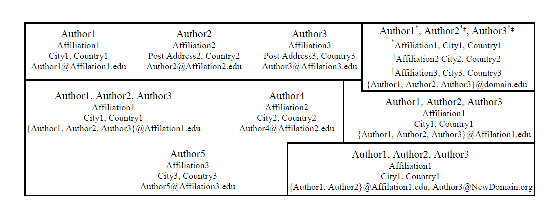
\includegraphics[width=0.45\textwidth]{Fig1}
	\caption{Different ways to design information about authors}
	\label{fig1}
\end{figure}

\section{Main part (Heading 1)}

\subsection{Structural components (Heading 2)}

\subsubsection{Introduction (Heading 3)}
The introduction it is a place for description of the problem, analysis of existing solutions (with links to sources), their disadvantages and  advantages of your approach. Clear statement of the work purpose is required.  

\subsubsection{Main part}
The main part is recommended to be divided into sections. The section titles should have meaningful names. The name ''Main part'' is not allowed.

\subsubsection{Lists}
There are two types of lists: bulleted and numbered. In numbered list use right bracket after number. 

%\begin{enumerate}
%	\item 
%\end{enumerate}

In bulleted list as a marker is using bullet. 

%\begin{itemize}
%	\item 
%\end{itemize}

If you start item from first word capitalized place at the end point, if not -- comma (or semicolon if in text of item comma have been used). At the end of last item place point.

\subsubsection{Equations}
Equations are numbered only if they are referenced in the text. 
\begin{equation}
	a-b=c
	\label{eq:1}
\end{equation}
where $a$ is main symbol, $b$ -- principal and $c$ -- basic.

Italicize Roman symbols for quantities and variables, but not Greek symbols. Use a long dash rather than a hyphen for a minus sign. Be sure that the symbols in your equation have been defined before or immediately following the equation.

Don't forget to use the same style for defining symbols in the text as in equation.

\subsubsection{Algorithms}
If you want to lead the algorithm, design it so Algorithm \ref{alg:algorithm}.

\begin{algorithm}
  \caption{Your algorithm}\label{alg:algorithm}
  \begin{algorithmic}
 
 \item Here will be the text of your algorithm. Make \textbf{operators} bold, variables \textit{italic}. step 1;
 \item step 2;
  \end{algorithmic}
\end{algorithm}

\section{Figures and tables}
Place figures and tables at the top and bottom of  page. Large figures and tables may span for all page. Them can be rotated if it is necessary. Each figure or table should be caption. Insert figures and tables after they are cited in the text. Use words rather than symbols or abbreviations when writing labels to avoid confusing the reader. Don't place point at the end of captions for figures or tables. 

\subsection{Figures}
Use the abbreviation ``Fig. 1'' in text. Use black and white colors, example of bad black and white graphics -- Fig. \ref{fig2}. Don't forget to attach to the source separate files with figures. Format EPS is mandatory for TeX source.

\begin{figure}[h]
	\centering
	
\includegraphics[width=0.45\textwidth]{Fig2}
	\caption{Red, blue and green line}
	\label{fig2}
\end{figure}

\subsection{Tables}

\begin{table}[h]
\centering
\label{tab1}
\caption{Popular drawbacks for submissions of FRUCT13}\label{tab1}\vspace{4pt}
\begin{tabular}{|c|c|c|c|}

		\hline
 		\textbf{Drawbacks in} & \textbf{Number of submissions} \\
 		\hline
		Paper Title & 7 \\
		\hline
		Information about authors & 10 \\
		\hline
		Abstract & 2 \\
		\hline
		Index Terms & 11 \\
		\hline
		Title of sections & 9 \\
		\hline
		General text & 10 \\
		\hline
		Figures and tables & 15 \\
		\hline
		Lists & 4 \\
		\hline
		References & 13 \\
		\hline
		Design do not match our template & 7 \\
		\hline
		In total & 40 \\
		\hline
\end{tabular}
\end{table}

\section{Design of references}

The template number citations consecutively within brackets \cite{Cover}. Numbering references depending on the order of their appearance in the text. The sentence punctuation follows the bracket \cite{Dobrushin}. Refer simply to the reference number, as in \cite{Blachman} -� do not use ``Ref. \cite{Blachman}'' or ``reference \cite{Blachman}'' except at the beginning of a sentence: ``Reference \cite{Blachman} was the first ...''

Unless there are six authors or more give all authors names; do not use ``et al.''. Papers that have not been published, even if they have been submitted for publication, should be cited as ``unpublished'' \cite{Elissa}. Papers that have been accepted for publication should be cited as ``in press'' \cite{Nicole}. Capitalize only the first word in a paper title, except for proper nouns and element symbols.

References must be design as a list. Use 9 point Times New Roman for References. In references there are two type of indent. First for references numbered from 1 to 9~-- indent from the left margin equal 0,4 cm and hanging indent for first line equal 0,6 cm. For all other~-- indent from the left margin equal 0,25 cm and hanging indent for first line equal 0,75 cm.

If you use \TeX, please, make references as in template in main file of \TeX  source. 

Requirements for formatting references are various depending on its type:
\begin{enumerate}
	\item Books
	
		\begin{itemize}
			\item Initials and family name of each authors by comma (at last use ``and'').
			\item Comma, \textit{name of book without quotes (italic)}, point at the end.
			\item Then all other bibliographic information by comma (publisher, year, page), point at the end.
		\end{itemize}	
		
		As example \cite{Cover}.
 	\item Articles
 
 		\begin{itemize}
			\item Initials and family name of each authors by comma.
			\item Comma, name of article in quotes, \textit{name of the journal or conference (italic)}.
			\item Then all other bibliographic information by comma (publisher, year, page), point at the end.
		\end{itemize}	
		
		Examples for article references in \cite{Dobrushin, Blachman}.
	\item Internet resources
	
 		\begin{itemize}
			\item Initials and family name of each authors by comma.
			\item Comma, name of intertet resource and other bibliographic information by comma (if exists).
			\item �Web:� and web link (not hyperlink), point at the end.
		\end{itemize}	
		
		Example -- \cite{IEEE}.
\end{enumerate}

\section{Conclusion}
This part presents the key findings in substance. Avoid simple enumeration of the following material. It is desirable to provide a link to existing articles and grants. 

\section*{Acknowledgment}
This section is not numbered. You may wish to express gratitude here.

\begin{thebibliography}{6}

\bibitem{Cover}
\textit{(Example for books)} T.M.Cover and J.A. Thomas, \emph{Elements of Information Theory}. New York: Wiley, 1991.

\bibitem{Dobrushin}
\textit{(Example for articles)} R.L. Dobrushin, ``Optimum information transmission through a channel with unknown parameters'',  \emph{Radiotech.Electron.}, vol.4, Dec.1959, pp. 1951-1956.

\bibitem{Blachman}
\textit{(Example for articles)} N.M. Blachman, ``Communication as a game'', \emph{in Proc. WESCON Conf.}, Aug. 1957, pp. 61-66.

\bibitem{IEEE}
\textit{(Example for web-links)} IEEE official website, Manuscript Templates for Conference Proceedings, Web: http://www.ieee.org/conferences\_events/conferences/publishing/templates.\newline html.

\bibitem{Elissa}
\textit{(Example for unpublished references)} K. Elissa, ``Title of paper if known'', unpublished.

\bibitem{Nicole}
\textit{(Example for references have been accepted for publication)} R. Nicole, ``Title of paper with only first word capitalized'', J. Name Stand. Abbrev., in press.

\end{thebibliography}

\end{document}